\section{Применение локального поиска для ускорения сходимости АГП}
Методы локального поиска могут применяться в сочетании с глобальными алгоритмами для улучшения полученных решений или текущих оценок оптимума.
В первом случае локальный метод стартует из точки, найденной глобальным методом, и уточняет решение практически до любой нужной точности. Это
позволяет избежать чрезмерных затрат на поиск решения с высокой точностью глобальным методом.
\par
Во втором случае локальный метод используется для ускорения обнаружения локальных оптимумов.
Информацилнно-статистический метод Стронгина позволяет обновлять свою поисковую информацию из любых посторонних источников, в том числе из точкек испытаний,
полученных от локального метода.
Как только глобальный метод находит новую оценку оптимума, из этой точки стартует локальный метод и все или часть испытаний, проведённых им
добавляется в поисковую информацию, далее глобальный метод продолжает работу. Каких-либо теоретических исследований подобной схемы не проводилось, поэтому её эффективность проверялась экспериментально.
\par
В качестве метода локальной оптимизации был выбран метод Хука-Дживса \cite{himmelblau}. Он прост в реализации и для его работы не требуется знать значений
 производных оптимизируемой функции.
\par
Были проведены две серии экспериментов, соответствующих следующим схемам добавления точек, полученных локальным методом в поисковую информацию:
\begin{itemize}
		\item добавление единственной точки, к которой сошёлся локальный метод;
    \item добавление всех промежуточных точек.
\end{itemize}
\par
Эксперименты проводились на классах GKLS 4d Simple и GKLS 5d Simple, параметры метода были заданы такие же, как в разделе \ref{sec:multilev_maps}
\begin{figure}[ht]
	\center
  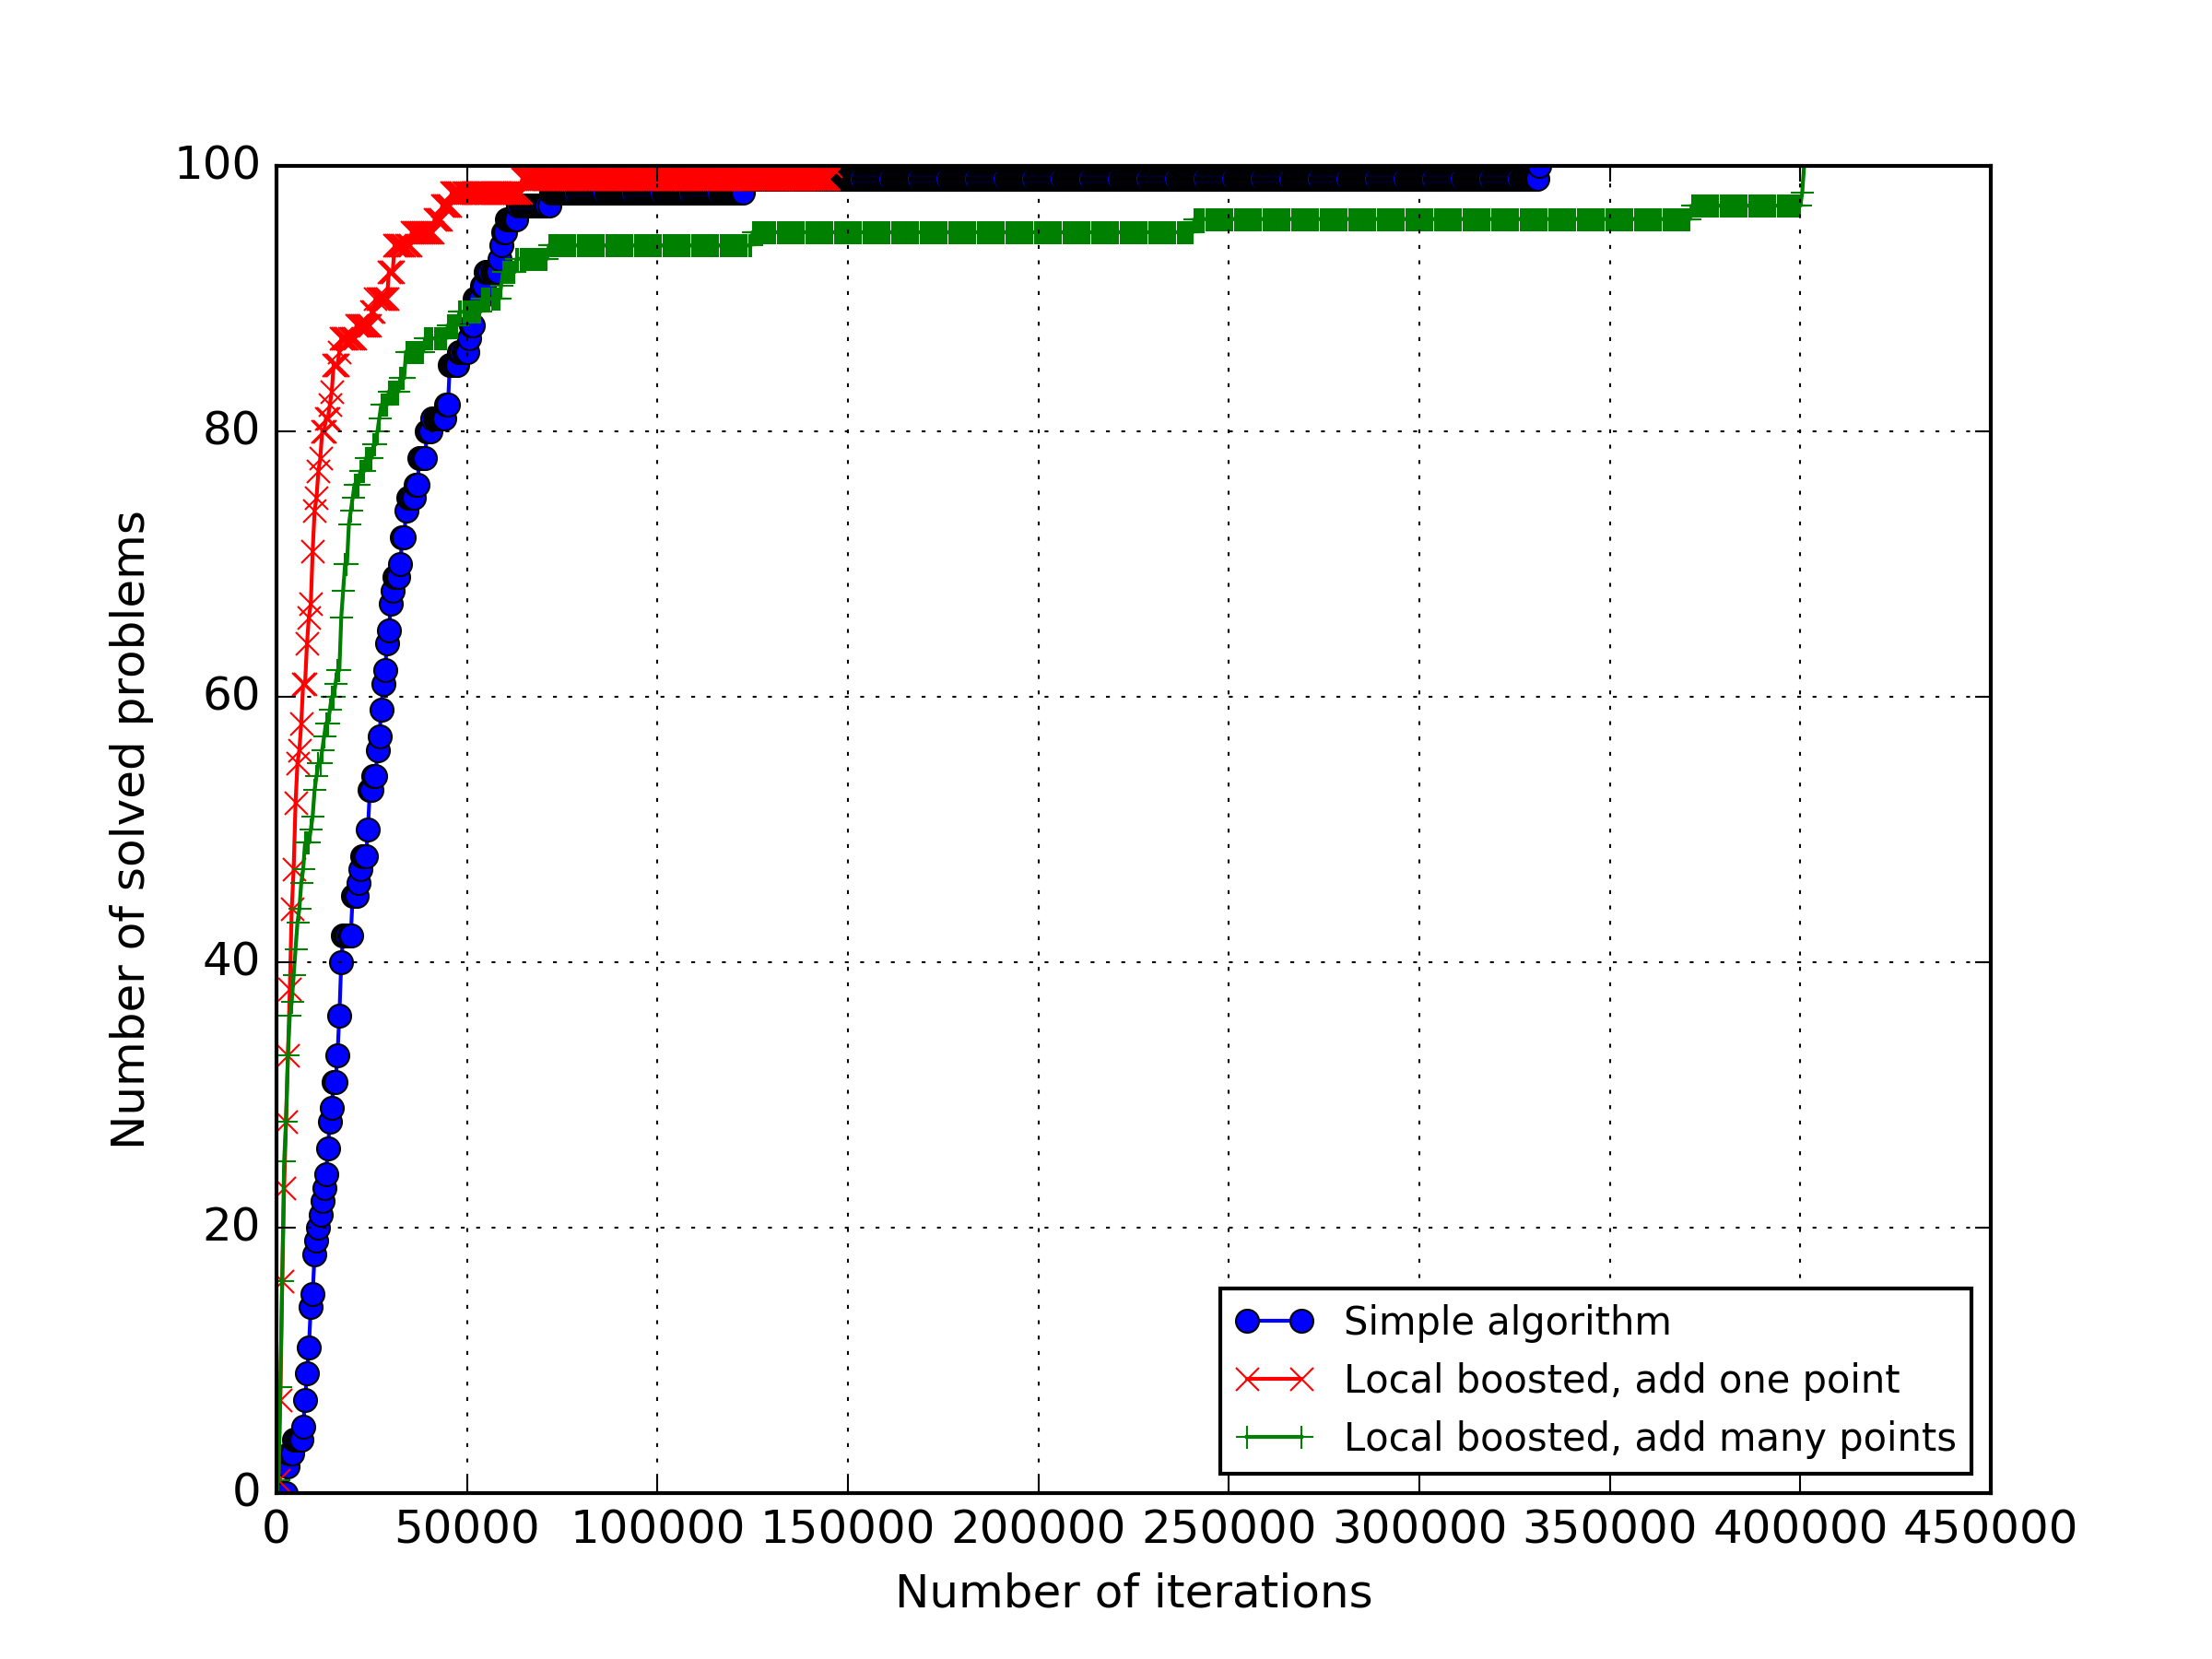
\includegraphics[width=0.75\textwidth]{pictures/local_search_op.png}
  \caption{Операционные характеристики на классе GKLS 4d Simple при различных вариантах использования локального метода}
  \label{fig:loaclsearchOP}
\end{figure}
Из рис. \ref{fig:loaclsearchOP}, \ref{fig:loaclsearchOP5d} можно сделать вывод, что вариант с использованием только одной лучшей точки, полученной локальным методом, оказался наилучшим.
В обоих случаях он заметно ускорил сходимость глобального алгоритма.
\begin{figure}[ht]
	\center
  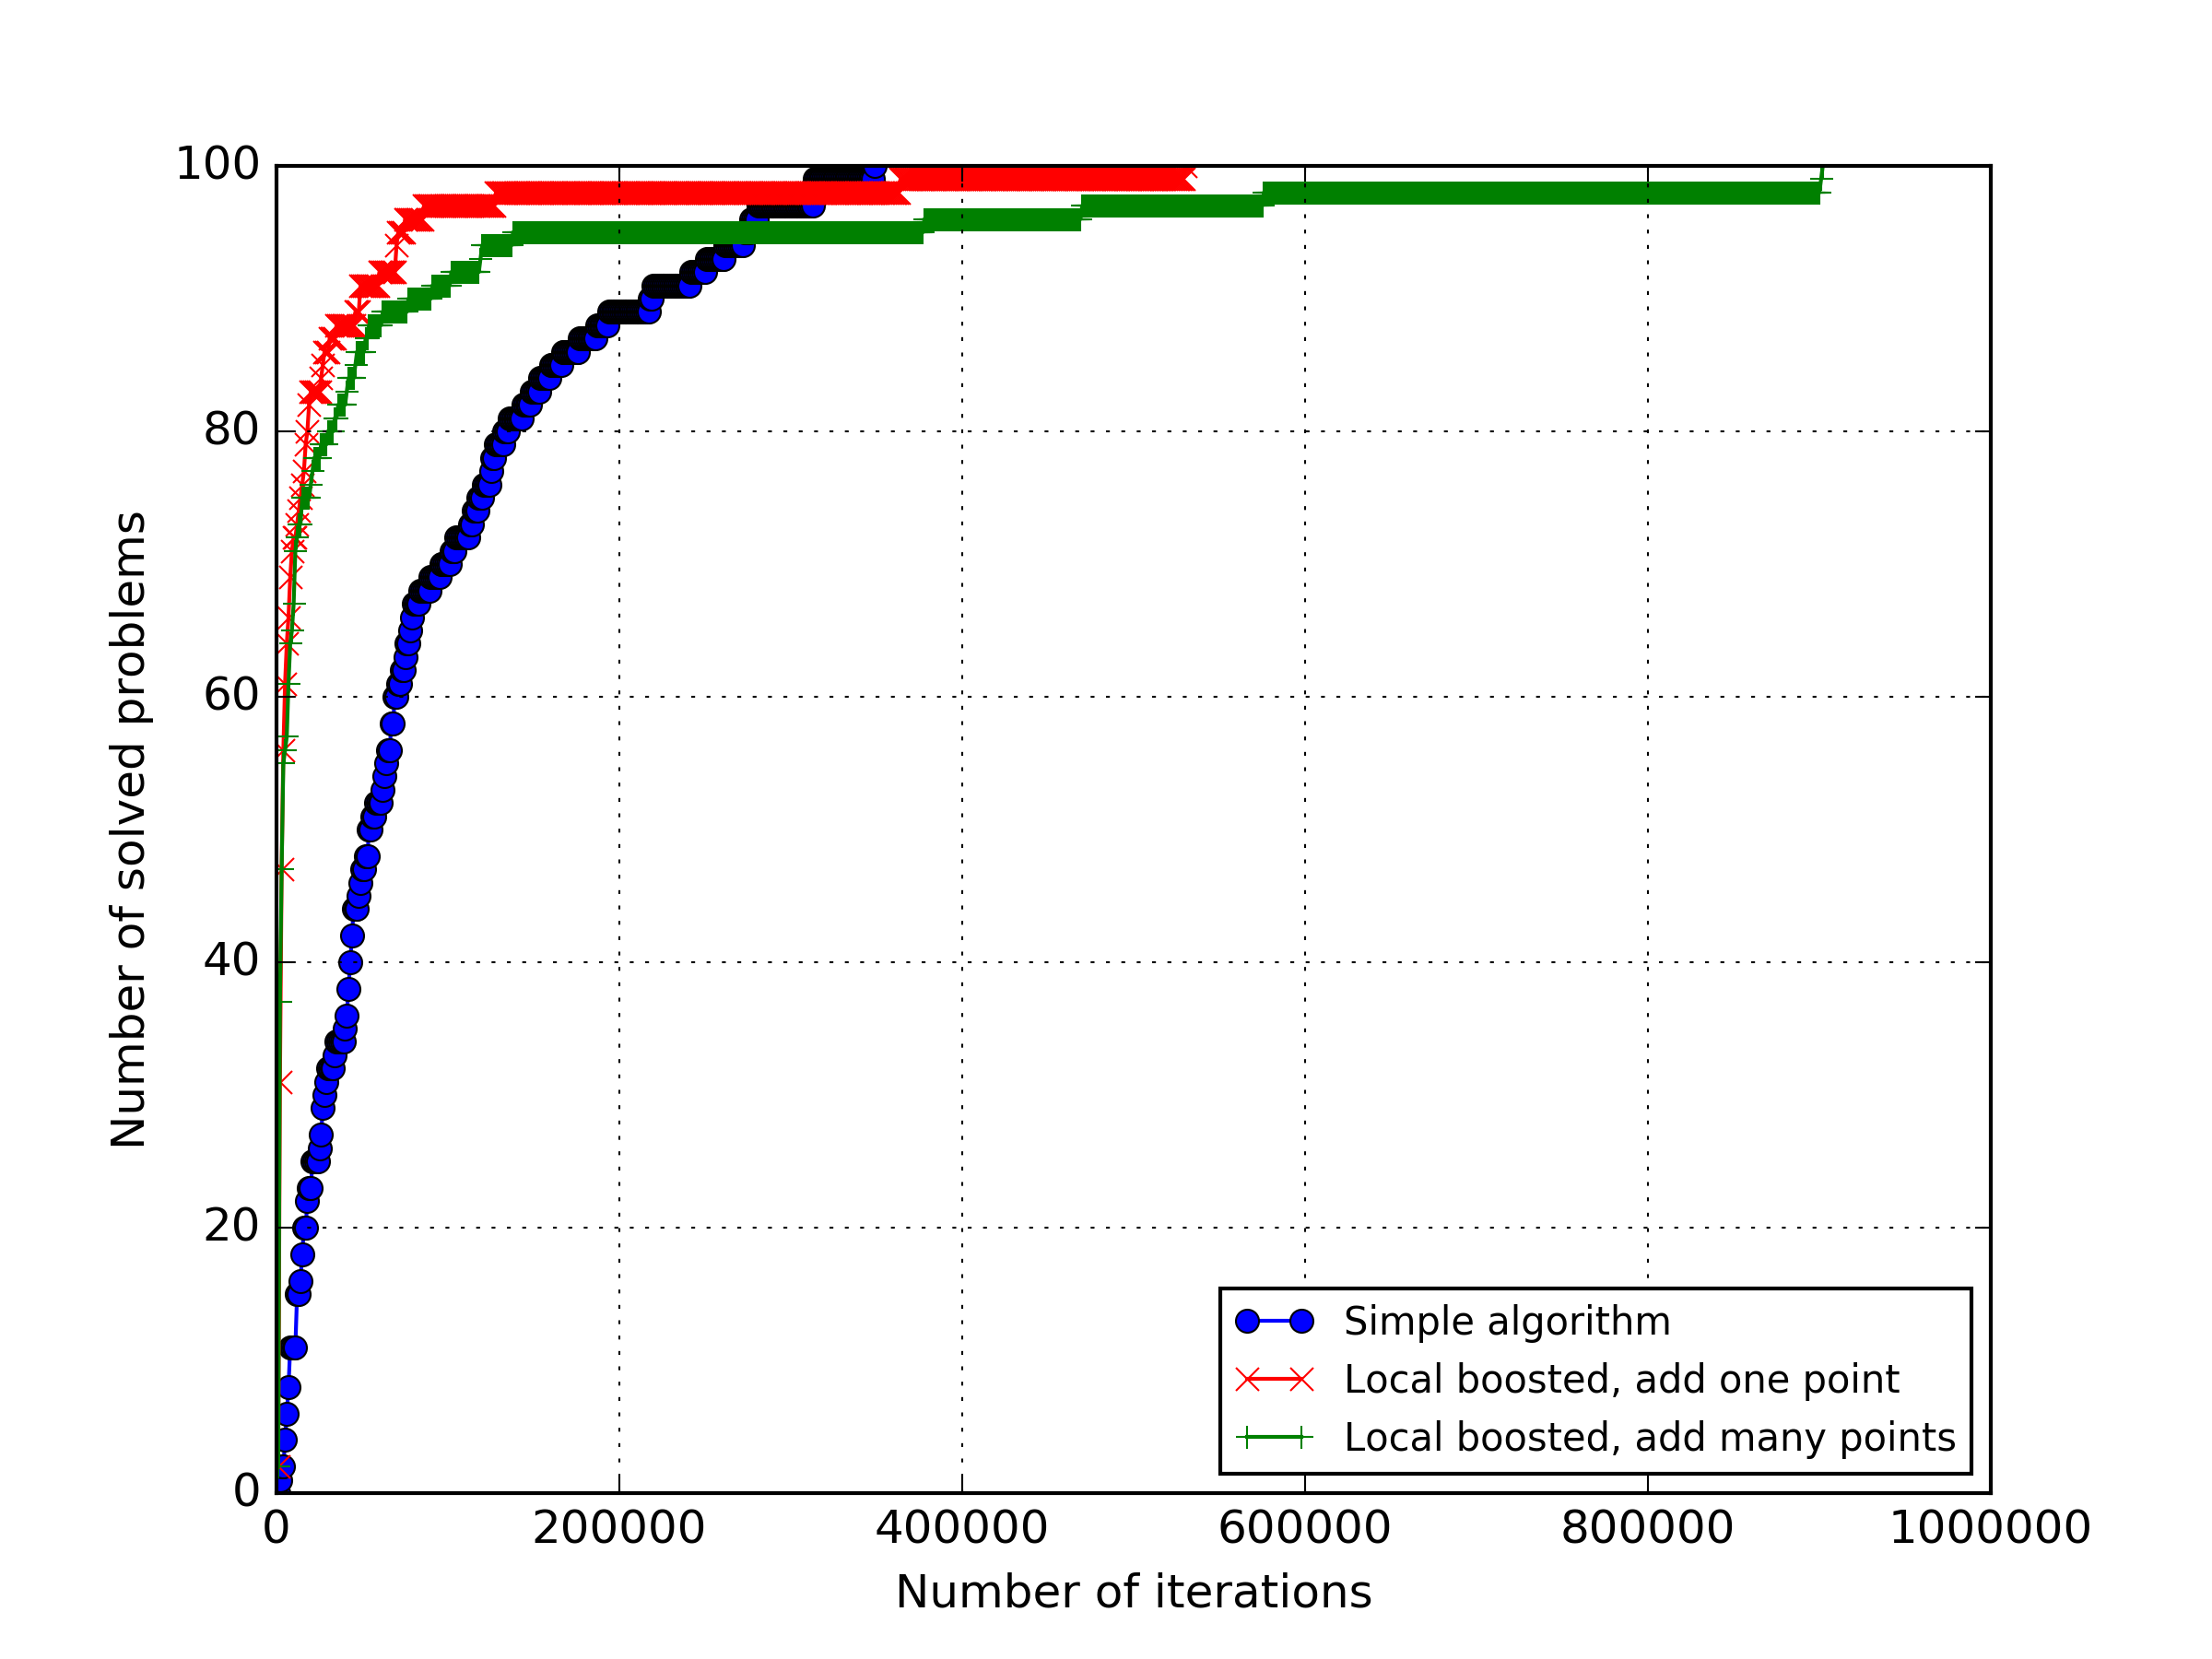
\includegraphics[width=0.75\textwidth]{pictures/local_search_op5d.png}
  \caption{Операционные характеристики на классе GKLS 5d Simple при различных вариантах использования локального метода}
  \label{fig:loaclsearchOP5d}
\end{figure}
